\documentclass{article}

\usepackage{geometry}
\geometry{
	a4paper,
	noheadfoot=true,
	left=1.0in,
	right=1.0in,
	top=1.0in,
	bottom=1.0in,
}
\usepackage[export]{adjustbox}
\usepackage[font={Large}]{caption}
\usepackage{hyperref}
\usepackage{xcolor}
\hypersetup{
    colorlinks,
    linkcolor={red!50!black},
    citecolor={blue!50!black},
    urlcolor={blue!80!black}
}

\newcommand\invisiblesection[1]{%
  \refstepcounter{section}%
  \addcontentsline{toc}{section}{\protect\numberline{\thesection}#1}%
  \sectionmark{#1}}

% https://tex.stackexchange.com/a/395713/109818
\newcommand{\mycaption}[2]{%
  \caption[#1]{\textbf{#1}\newline\normalsize#2}%
}

% list of figures spacing between number and caption
\usepackage{tocloft}
\setlength{\cftfignumwidth}{4em}
% spacing in list of figures
\setlength\cftbeforefigskip{\baselineskip}

\begin{document}

% no page numbering
\pagenumbering{gobble}
\begingroup
  \centering
  \LARGE \href{https://github.com/FanWangEcon/Tex4Econ/tree/master/template/fantemplate_image_appendix}{Tables and Figures Appendix} for \\[1.0em]
   Template File for Tables and Figures Appendix \\[1.0em]
  \large \href{http://fanwangecon.github.io/}{Fan Wang} \\[0.5em]
  \large \today \\[1.0em]\par
\endgroup

\listoffigures

\pagebreak
\clearpage

% From: https://tex.stackexchange.com/a/110908/109818
\begin{figure}[h]
\mycaption{Scatter Plot QSEC HP}{This is a testing file from \href{https://fanwangecon.github.io/Tex4Econ/}{Tex4Econ} for a PDF file including only images, designed as an add-on Appendix to a File Generated Elsewhere, by Word, for example. Font size for capture is controlled by the Caption package's font option. Image can bleed into 1 inch margin, and is centered using makebox. This is the first image. This image is on top with figure \textit{h} option. Note also that this page does not have a page number, deleted with \textit{gobble}. Also note this has a caption heading and a caption detail. The caption details do not appear in the list of figures. See Figures \ref{fig:image2} and \ref{fig:image3}. \label{fig:image1}}
\hspace*{-\dimexpr\oddsidemargin+1in\relax}
\makebox[\paperwidth]{%
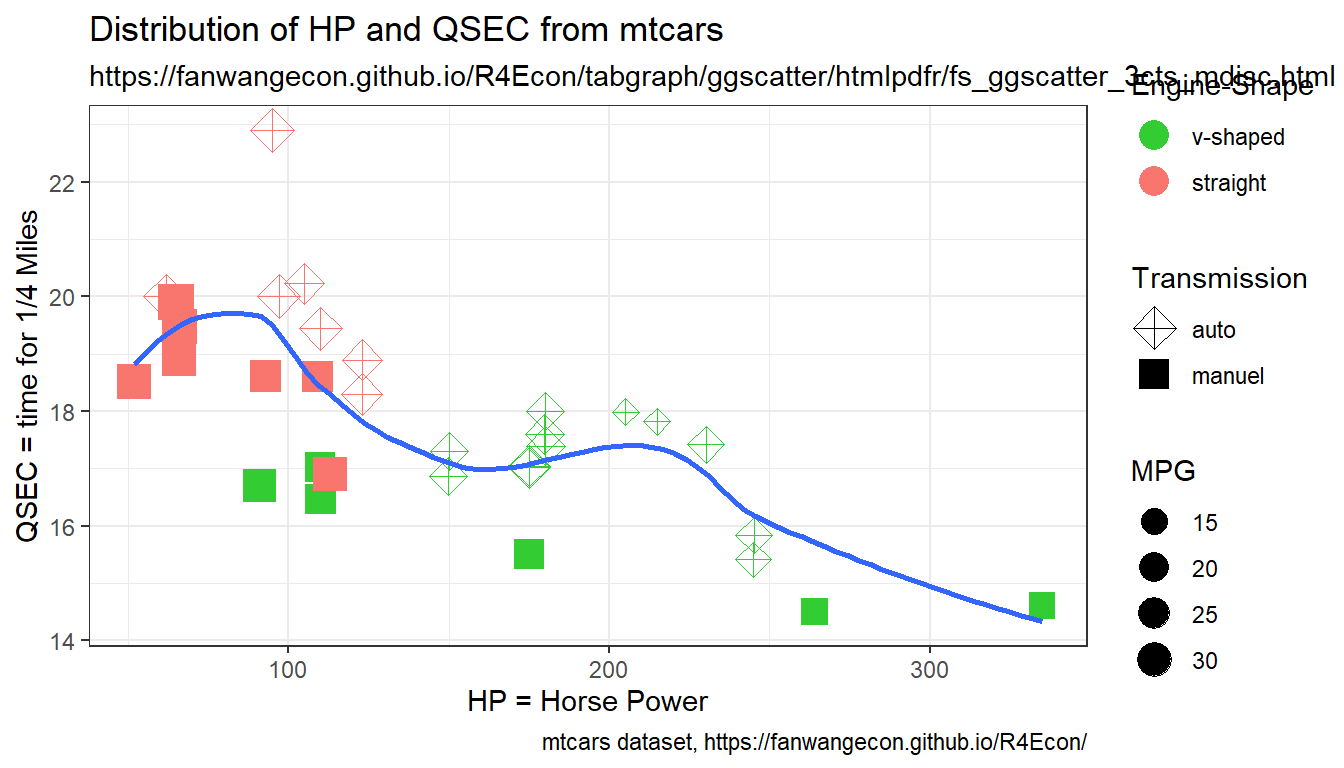
\includegraphics[width=1.1\textwidth]{img/img1.png}
}
\hspace*{-\paperwidth}
\end{figure}

\pagebreak
\clearpage

% start page-numbering
\pagenumbering{arabic} 
\setcounter{page}{26}

\begin{figure}[p]
\hspace*{-\dimexpr\oddsidemargin+1in\relax}
\makebox[\paperwidth]{%
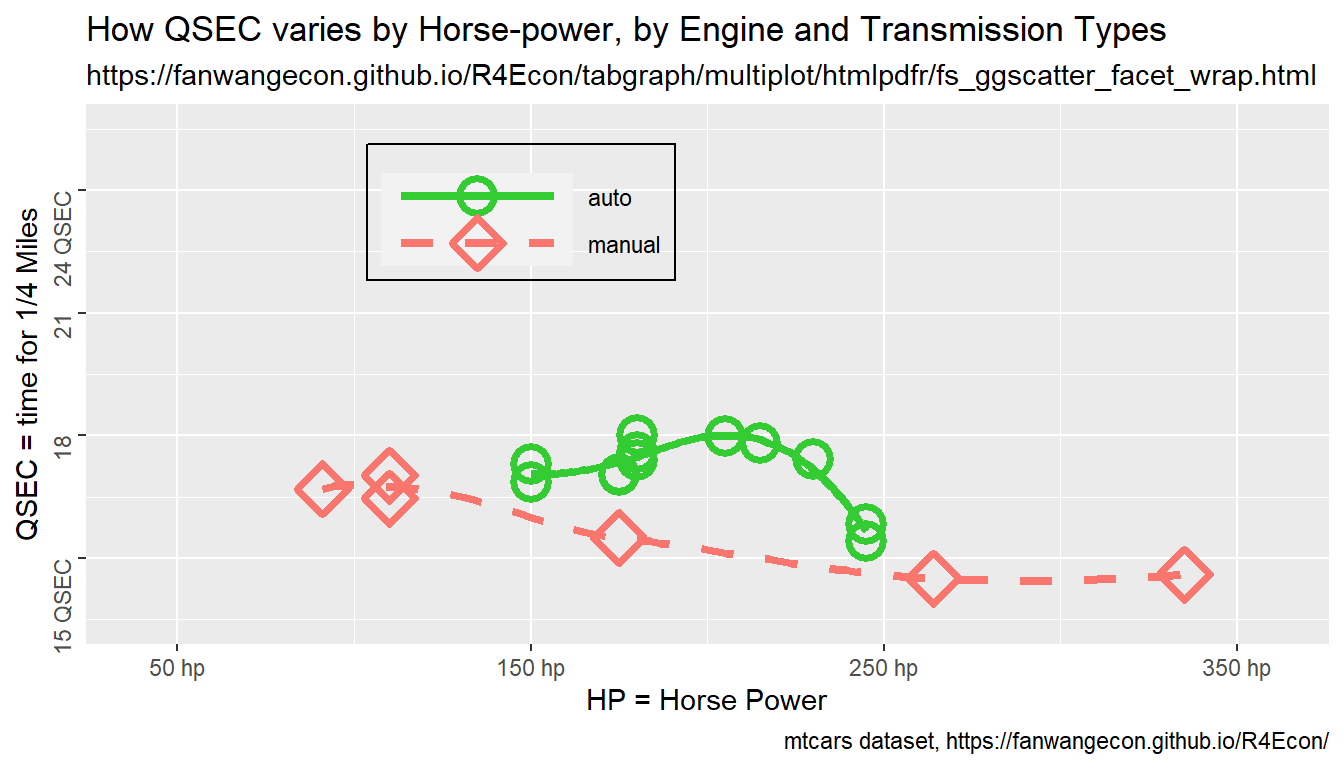
\includegraphics[width=1.0\textwidth]{img/img2.png}
}
\mycaption{QSEC and HP Two Lines}{This is a testing file from \href{https://fanwangecon.github.io/Tex4Econ/}{Tex4Econ} for a PDF file including only images, designed as an add-on Appendix to a File Generated Elsewhere. This is the second image, centered on the page, and does not bleed into 1 inch margin. Note that the page number is set at 26. See Figures \ref{fig:image1} and \ref{fig:image3}. \label{fig:image2}}
\hspace*{-\paperwidth}
\end{figure}

\pagebreak
\clearpage


% start page-numbering
\pagenumbering{arabic} 
\setcounter{page}{1}

\begin{figure}[p]
\caption{A Standard Caption with Hidden Caption Below Text. This is a testing file from \href{https://fanwangecon.github.io/Tex4Econ/}{Tex4Econ} for a PDF file including only images. \label{fig:image3}}
\hspace*{-\dimexpr\oddsidemargin+1in\relax}
\makebox[\paperwidth]{%
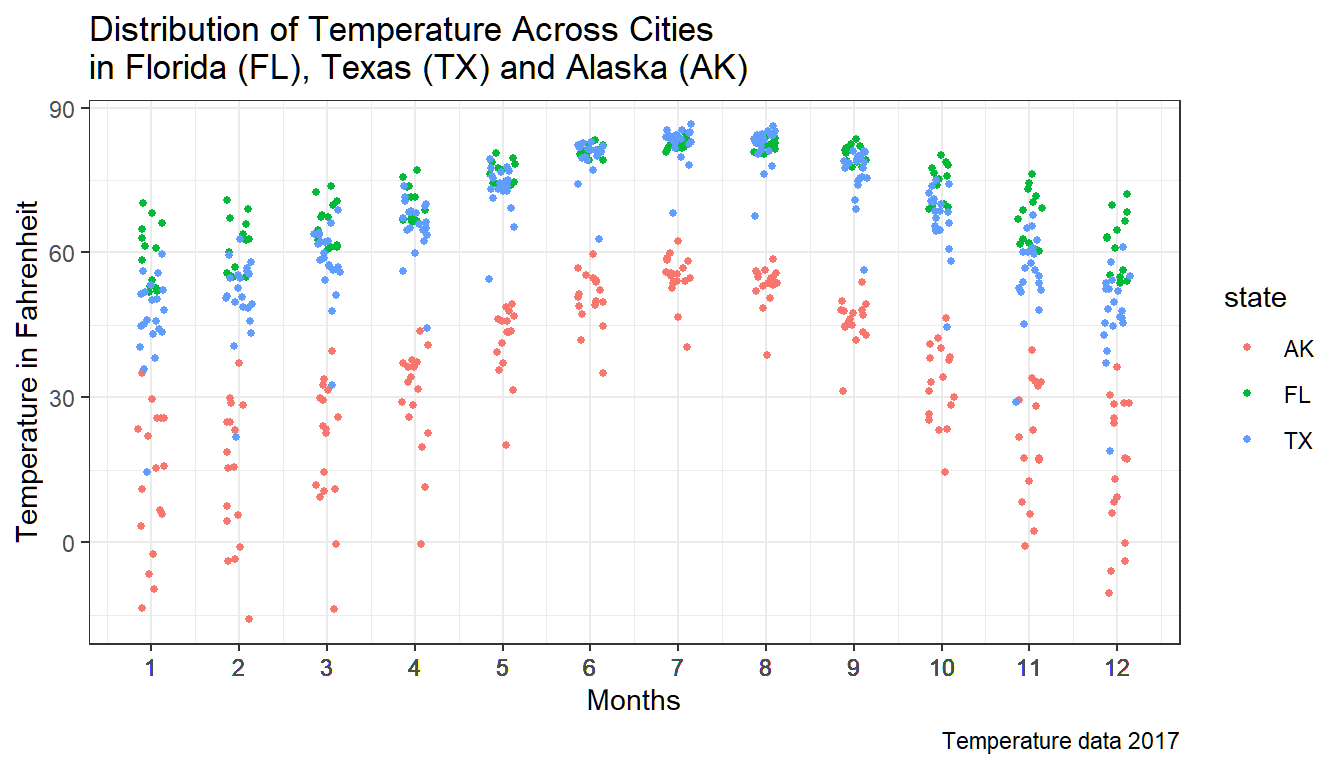
\includegraphics[width=0.95\paperwidth]{img/img3.png}
}
\caption*{This is a testing file from \href{https://fanwangecon.github.io/Tex4Econ/}{Tex4Econ} for a PDF file including only images, designed as an add-on Appendix to a File Generated Elsewhere. This is the third image, with caption on top. And the image bleeds into the margins by matching paperwidth 95 percent. Image also centered on page. Note that the page number is set at 1. Note this is a standard caption. See Figures \ref{fig:image1} and \ref{fig:image2}.}
\hspace*{-\paperwidth}
\end{figure}

\invisiblesection{One}
\setcounter{figure}{0}
\renewcommand{\thefigure}{A.\arabic{section}.\arabic{figure}}

\begin{figure}[p]
\caption{A standard caption without additional bottom notes. Cash-on-Hand Period t and t+1. This Figure is number with a section number from an invisible section. The A and B might represent Appendix names. See Figure \ref{fig:image5}. \label{fig:image4}}
\hspace*{-\dimexpr\oddsidemargin+1in\relax}
\makebox[\paperwidth]{%
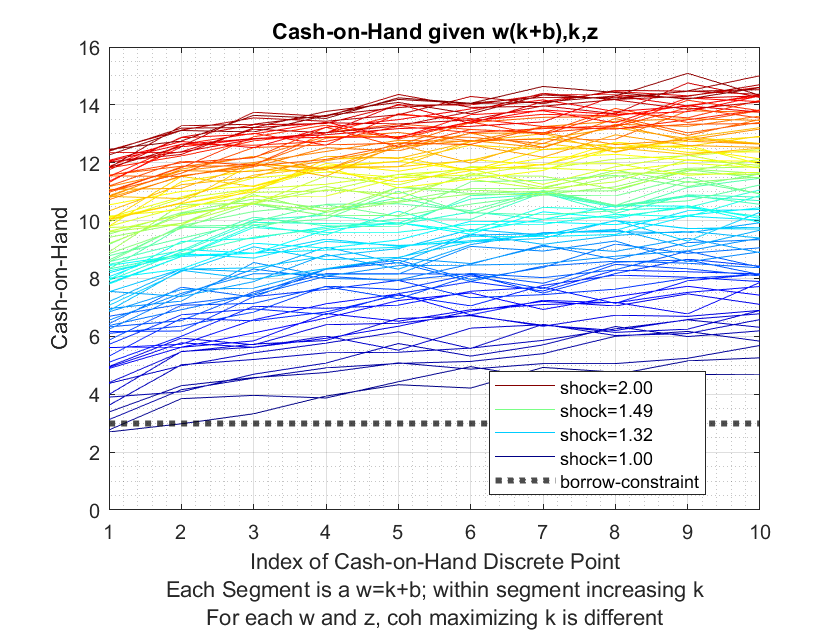
\includegraphics[width=1.0\textwidth]{img/img4.png}
}
\hspace*{-\paperwidth}
\end{figure}

\invisiblesection{Two}
\renewcommand{\thefigure}{B.\arabic{section}.\arabic{figure}}
\setcounter{figure}{0}

\begin{figure}[p]
\mycaption{Asset Choice Grids}{This Figure is number with a different section number from an invisible section. The A and B might represent Appendix names. See Figure \ref{fig:image4}. \label{fig:image5}}
\hspace*{-\dimexpr\oddsidemargin+1in\relax}
\makebox[\paperwidth]{%
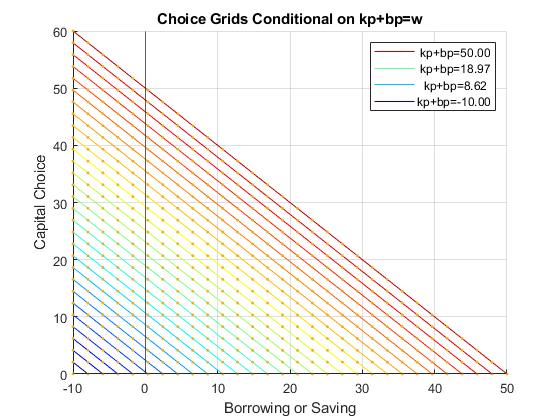
\includegraphics[width=1.0\textwidth]{img/img5.png}
}
\hspace*{-\paperwidth}
\end{figure}


\end{document}
